\paragraph{} \ac{RNA} é uma classe de modelos de aprendizado de máquina inspirados no funcionamento do cérebro humano, sendo capazes de aprender e tomar decisões com base em amostras apresentados durante o processo de treinamento \cite{haykin1998neural}. A partir dessas amostras, as redes neurais generalizam o aprendizado para dados previamente desconhecidos, permitindo que realizem inferências sobre novos conjuntos de dados.

\paragraph{} As \ac{RNA}s são geralmente estruturadas em três tipos de camadas: camada de entrada, camadas ocultas (ou de processamento) e camada de saída. Essas camadas podem ser organizadas de diversas maneiras, formando topologias específicas que variam de acordo com a aplicação. À medida que os dados de entrada percorrem as camadas da rede, eles são transformados progressivamente por meio de funções de ativação e ajustes sinápticos, que determinam a força das conexões entre os neurônios.

\paragraph{} O ajuste dos pesos sinápticos ocorre durante o processo de treinamento, em que algoritmos de otimização, como o método do gradiente descendente, são utilizados para minimizar o erro entre a saída prevista e a saída desejada. A retropropagação do erro é uma técnica amplamente utilizada para este fim, ajustando os pesos de forma iterativa e eficiente, garantindo a convergência para uma solução ótima.

\paragraph{} Quando uma rede neural recebe um vetor de entrada \(x\), ela realiza cálculos que geram uma saída \(y\), de acordo com a Equação \ref{eq:nn}:

\begin{equation}
	y = f(Wx + b)
	\label{eq:nn}
\end{equation}

\paragraph{} Nesta equação, \(W\) representa a matriz de pesos sinápticos da rede, \(b\) corresponde ao vetor de viés ajustado durante o treinamento, e \(f\) é a função de ativação, responsável por introduzir não linearidades no modelo. A saída \(y\) é, portanto, o resultado final do processamento, obtido após a aplicação dessas transformações.

\section{Perceptron de Rosenblatt}

\paragraph{} O Perceptron, introduzido por Rosenblatt, 1958 \cite{rosenblatt1958perceptron}, foi um dos primeiros modelos de rede neural e representa um marco no desenvolvimento da inteligência artificial. Ele foi concebido para realizar tarefas de classificação linear, sendo capaz de separar classes de dados que são linearmente separáveis. O modelo Perceptron é composto por um único neurônio, que processa um conjunto de entradas, cada uma associada a um peso sináptico, e produz uma saída binária com base em uma função de ativação \cite{rosenblatt1958perceptron}.

\paragraph{} O funcionamento do Perceptron é descrito da seguinte forma:

\begin{equation}
	y = \begin{cases}
		1, & \text{se } \sum_{i=1}^{n} w_i x_i + b > 0 \\
		0, & \text{caso contrário}
	\end{cases}
\end{equation}

\paragraph{} Sendo \(x_i\) as entradas do modelo, \(w_i\) os pesos sinápticos associados a cada entrada, \(b\) o viés (bias) do modelo, ajustável durante o treinamento, e \(y\) a saída binária do Perceptron.

\subsection{Limitações e Extensões}

\paragraph{} Embora o Perceptron tenha sido um avanço significativo, ele é limitado a problemas que podem ser separados por uma linha reta (ou hiperplano no caso de dimensões superiores), ou seja, dados que são linearmente separáveis. Em 1969, Minsky e Papert \cite{minsky1969perceptrons} demonstraram que o Perceptron era incapaz de resolver problemas como o XOR, que não são linearmente separáveis. Essa limitação levou à introdução de arquiteturas mais complexas, como o \ac{MLP}, que supera essa deficiência ao incorporar camadas ocultas e ativação não linear \cite{minsky1969perceptrons}.

\paragraph{} O Perceptron de Rosenblatt foi fundamental para o desenvolvimento posterior de redes neurais e permanece como um conceito básico no aprendizado de máquina.

\paragraph{} O treinamento do Perceptron utiliza uma regra de aprendizado simples e eficiente, conhecida como regra do Perceptron \cite{rosenblatt1958perceptron}. Para cada amostra de treinamento, os pesos são ajustados de acordo com o erro entre a saída prevista e a saída desejada:

\begin{equation}
	w_{i}(t+1) = w_{i}(t) - \eta \frac{\partial E}{\partial w_{i}(t)}
\end{equation}
\paragraph{} Sendo \(w_{i}(t)\) o peso sináptico do neurônio \(i\) no instante \(t\), \(\eta\) a taxa de aprendizado, que controla o tamanho do passo de ajuste e\(\frac{\partial E}{\partial w_{i}(t)}\) o gradiente do erro em relação ao peso.

\paragraph{} Essa regra de atualização ajusta os pesos para reduzir o erro de classificação em cada iteração.

\section{Treinamento de Redes Neurais}

\paragraph{} O treinamento das redes neurais consiste na apresentação dos dados de entrada, acompanhados das respectivas saídas desejadas (supervisionado), ou simplesmente dos dados de entrada no caso de aprendizagem não supervisionada. Durante o treinamento, o objetivo principal é minimizar a função de perda, que avalia  as saídas previstas pela rede com base nas saídas reais.

\paragraph{} O algoritmo mais comum para esse ajuste é o gradiente descendente, que atualiza os pesos sinápticos conforme a direção de maior declínio do erro. Métodos como o gradiente estocástico, Adam e RMSprop são variações amplamente utilizadas, aprimorando o desempenho em diferentes cenários.

\subsection{Retropropagação}

\paragraph{} A retropropagação  é o algoritmo mais utilizado para o treinamento de redes neurais supervisionadas. Introduzido por Rumelhart et al, 1986 \cite{rumelhart1986learning}, esse algoritmo ajusta os pesos sinápticos da rede para minimizar o erro entre a saída prevista e a saída desejada, utilizando o gradiente descendente.

\paragraph{} A retropropagação ocorre em duas fases principais, mostradas na Figura \ref{fig:mlp_diagram_backprop} e detalhadas a seguir:

\begin{figure}
	\begin{center}
		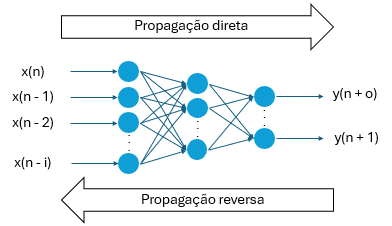
\includegraphics[width=0.8\textwidth]{figuras/mlp_diagram_backprop.png}
		\caption{Diagrama da \acs{MLP} nas fases de retropropagação}
		\label{fig:mlp_diagram_backprop}
		\text{Fonte: Elaborado pelo autor, baseado em \cite{haykin1998neural, rumelhart1986learning}}
	\end{center}
\end{figure}

\begin{itemize}
	\item \textbf{Fase de propagação direta}: Os dados de entrada são propagados pela rede, camada por camada, até que a saída seja calculada. Esta saída é então comparada com o valor esperado, e o erro é calculado com base em uma função de perda, como o \ac{MSE} ou a entropia cruzada.
	\item \textbf{Fase de propagação reversa}: O erro calculado é retropropagado da camada de saída para as camadas anteriores, ajustando os pesos sinápticos de acordo com o gradiente do erro em relação a cada peso. O objetivo é reduzir o erro a cada iteração, tornando o modelo mais preciso.
\end{itemize}

\paragraph{} A atualização dos pesos é dada pela seguinte equação:

\begin{equation}
	w_{ij}(t+1) = w_{ij}(t) - \eta \frac{\partial F_o}{\partial w_{ij}(t)}
\end{equation}
\paragraph{} Sendo \(w_{ij}(t)\) o peso sináptico entre o neurônio \(i\) e o neurônio \(j\) no instante \(t\), \(\eta\) a taxa de aprendizado, que controla o tamanho do passo de ajuste e \(\frac{\partial F_o}{\partial w_{ij}(t)}\) o gradiente da função objetivo em relação ao peso.

\paragraph{} A retropropagação é eficaz em problemas complexos, permitindo o ajuste eficiente dos parâmetros, mas pode enfrentar desafios como o problema do gradiente desaparecendo, que pode ser mitigado com técnicas como funções de ativação como a \ac{ReLU} e o uso de redes profundas com inicializações adequadas de peso.

\section{Funções de Ativação}

\paragraph{} As funções de ativação são elementos essenciais nas redes neurais, pois introduzem não linearidade no modelo, permitindo que ele aprenda padrões complexos. Entre as funções de ativação mais utilizadas estão:

\begin{itemize}
	\item \textbf{Sigmoide}:
	      \begin{equation}
		      f(x) = \frac{1}{1 + e^{-x}}
	      \end{equation}

	      \paragraph{} É utilizada principalmente em saídas binárias, transformando valores reais em probabilidades entre 0 e 1.
	\item \textbf{\ac{ReLU}}:
	      \begin{equation}
		      f(x) = \max(0, x)
	      \end{equation}

	      \paragraph{} Amplamente utilizada em redes profundas por sua simplicidade e eficiência computacional.
	\item \textbf{Tanh}:
	      \begin{equation}
		      f(x) = \frac{e^x - e^{-x}}{e^x + e^{-x}}
	      \end{equation}

	      \paragraph{} A função tangente hiperbólica, semelhante à sigmoide, mas com saída no intervalo \([-1, 1]\).

	\item \textbf{Softmax}:
	      \begin{equation}
		      f(x_i) = \frac{e^{x_i}}{\sum_{j=1}^{n} e^{x_j}}
	      \end{equation}

	      \paragraph{} Usada em problemas de classificação multiclasse, transformando um vetor de valores em probabilidades.
\end{itemize}


\section{Arquiteturas}

As redes neurais podem assumir diferentes arquiteturas, de acordo com o problema que se busca resolver. A seguir, algumas das principais arquiteturas:

\begin{itemize}

	\item \textbf{\acf{NARX}}: A rede \ac{NARX} é uma arquitetura específica de redes neurais utilizada para modelagem de séries temporais, onde a saída depende não apenas das entradas passadas, mas também de saídas anteriores. Ela é amplamente aplicada em sistemas dinâmicos.

	\item \textbf{\acf{RNN}}: As \acp{RNN} possuem conexões entre os neurônios que permitem o processamento sequencial de dados, tornando-as adequadas para tarefas como modelagem de séries temporais, reconhecimento de fala e tradução automática.

	\item \textbf{\acf{MLP}}: O \ac{MLP} é uma das arquiteturas mais clássicas e simples de redes neurais, composta por múltiplas camadas de neurônios com conexões completas entre si. É utilizado principalmente para problemas de classificação e regressão.

	\item \textbf{Redes Morfológicas}: As redes neurais morfológicas utilizam operadores matemáticos morfológicos no lugar de funções de ativação tradicionais. Elas são especialmente úteis para tarefas de processamento de imagens, onde operações como dilatação e erosão são comuns.

	\item \textbf{Redes Profundas}: As Redes Neurais Profundas são caracterizadas por terem múltiplas camadas ocultas, permitindo a aprendizagem de representações mais complexas e abstratas dos dados. Elas são amplamente utilizadas em áreas como reconhecimento de imagens e processamento de linguagem natural. A profundidade da rede permite a extração de características de alto nível, o que é fundamental para o sucesso em tarefas como a classificação de imagens e tradução automática.

\end{itemize}
